\section{Discrepancies and Ambiguities}
\label{discrep}

% Moved earlier to display nicely in paper
% \discrepClssTable{}
% \discrepCatsTable{}

After gathering all these data\footnote{Available in \texttt{ApproachGlossary.csv}
    and \texttt{QualityGlossary.csv} at \ifblind{[Repository link suppressed]}
    {\url{https://github.com/samm82/TestGen-Thesis}}.}, we found many
discrepancies. To better understand and analyze these discrepancies, each one
is given a ``class'' and a ``category''. \nameref{discrepClasses} describe
\emph{how} a discrepancy manifests syntactically; examples include \nameref{wrong}
and \nameref{miss}. On the other hand, \nameref{discrepCategories} describe the
knowledge domain in which a discrepancy manifests semantically; examples include
\nameref{syns} and \nameref{pars}. Within these sections, \ifnotpaper ``more
    significant'' discrepancies are listed first, followed by ``less significant''
    ones omitted from the paper version of this thesis for brevity. They are
    then \else discrepancies are \fi sorted based on their
\hyperref[sources]{source category}.

A summary of how many discrepancies there are by class and by category is shown
in \Cref{tab:discrepClss,tab:discrepCats}, respectively, where a given row
corresponds to the number of discrepancies either within that
\hyperref[sources]{source category} and/or with a ``more trusted'' one
(i.e., a previous row in the table). The numbers of (Exp)licit and (Imp)licit
(see \Cref{rigidity}) discrepancies are also presented in these tables. Note
that all manually tracked discrepancies appear in \emph{both}
\Cref{discrepClasses,discrepCategories}, while those
\hyperref[auto-discrep-analysis]{automatically} uncovered based on semantics
are only listed in their appropriate \hyperref[discrepCategories]{category} for
clarity (but still contribute to the counts in \Cref{tab:discrepClss}).

Additionally, specific subsets of testing presented significant issues. These
are given in their specific sections to keep related information together.
These discrepancies still count towards one or more of the categories of
discrepancies listed above\ifnotpaper; \Cref{aug-discrep-analysis} outlines how
this is done\fi. The ``problem'' subsets of testing include
\nameref{func-test-discrep}, \ifnotpaper\nameref{oat-discrep}, \fi
\nameref{recov-discrep}, \nameref{scal-discrep}, and \nameref{compat-discrep}.
\ifnotpaper Finally, \nameref{infer-discreps} are also given for completeness,
    despite being less certain and thus not contributing to any counts.

    \begin{bigLandscape}
        \discrepClssTable{}
        \discrepCatsTable{}
    \end{bigLandscape}

    \begin{figure*}
\centering
\begin{subfigure}[t]{0.475\textwidth}
\begin{tikzpicture}[thick, scale=0.7, every label/.style={align=left, scale=0.7}]
   \pie[text=legend, sum=auto, hide number, color={blue!60, cyan!60, yellow!60}]{
      25/48.1\%,
      22/42.3\%,
      5/9.6\%
}
\end{tikzpicture}
\caption{Discrepancies found in \stds{}.}
\label{fig:stdDiscrepSources}
\end{subfigure}
\hfill
\begin{subfigure}[t]{0.475\textwidth}
\begin{tikzpicture}[thick, scale=0.7, every label/.style={align=left, scale=0.7}]
   \pie[text=legend, sum=auto, hide number, color={blue!60, yellow!60, orange!60}]{
      24/38.1\%,
      29/46\%,
      10/15.9\%
}
\end{tikzpicture}
\caption{Discrepancies found in \metas{}.}
\label{fig:metaDiscrepSources}
\end{subfigure}
\vskip\baselineskip
\begin{subfigure}[t]{0.475\textwidth}
\begin{tikzpicture}[thick, scale=0.7, every label/.style={align=left, scale=0.7}]
   \pie[text=legend, sum=auto, hide number, color={blue!60, yellow!60, orange!60, red!60}]{
      7/21.9\%,
      13/40.6\%,
      7/21.9\%,
      5/15.6\%
}
\end{tikzpicture}
\caption{Discrepancies found in \texts{}.}
\label{fig:textDiscrepSources}
\end{subfigure}
\hfill
\begin{subfigure}[t]{0.475\textwidth}
\begin{tikzpicture}[thick, scale=0.7, every label/.style={align=left, scale=0.7}]
   \pie[text=legend, sum=auto, hide number, color={blue!60, yellow!60, orange!60, red!60, blue!60!cyan!60}]{
      14/26.9\%,
      17/32.7\%,
      14/26.9\%,
      3/5.8\%,
      4/7.7\%
}
\end{tikzpicture}
\caption{Discrepancies found in \papers{}.}
\label{fig:paperDiscrepSources}
\end{subfigure}
\vskip\baselineskip
\begin{center}
\begin{subfigure}[t]{\linewidth}
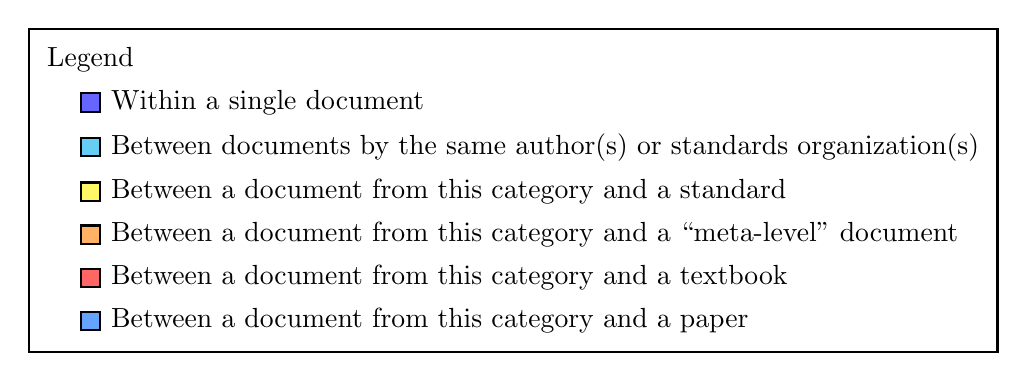
\begin{tikzpicture}
\matrix [thick, draw=black] {
\node[label=center:Legend] {{}}; \\
\node[thick, shape=rectangle, draw=black, fill=blue!60, label=right:{Within a single document}](0) {}; \\
\node[thick, shape=rectangle, draw=black, fill=cyan!60, label=right:{Between documents by the same author(s) or standards organization(s)}](1) {}; \\
\node[thick, shape=rectangle, draw=black, fill=yellow!60, label=right:{Between a document from this category and a standard}](2) {}; \\
\node[thick, shape=rectangle, draw=black, fill=orange!60, label=right:{Between a document from this category and a ``meta-level'' document}](3) {}; \\
\node[thick, shape=rectangle, draw=black, fill=red!60, label=right:{Between a document from this category and a textbook}](4) {}; \\
\node[thick, shape=rectangle, draw=black, fill=blue!60!cyan!60, label=right:{Between a document from this category and a paper}](5) {}; \\
};
\end{tikzpicture}
\end{subfigure}
\end{center}
\hfill
\caption{Sources of discrepancies based on \hyperref[sources]{source category}.}
\label{fig:discrepSources}
\end{figure*}
 \fi

\subsection{Discrepancy Classes}
\label{discrepClasses}

The following sections list observed discrepancies grouped by \emph{how} the
discrepancy manifests. These include \nameref{wrong}, \nameref{miss},
\nameref{contra}, \nameref{ambi}, \nameref{over}, and \reduns{}.

\subsubsection{Mistakes}
\label{wrong}
The following are cases where information is incorrect; this includes cases
\terms{} included that should \emph{not} have been, untrue claims about
\cites{}, and simple typos:

\input{build/DiscrepClsWrong}

\subsubsection{Omissions}
\label{miss}
The following are cases where information (usually \defs{}) \emph{should have}
been included but was not:

\input{build/DiscrepClsMiss}

\subsubsection{Contradictions}
\label{contra}
The following are cases where multiple sources of information (sometimes within
the same document!) disagree; note that cases where all sources of information
are incorrect are considered contradictions and not \nameref{wrong}, since this
would require analysis that has not been performed yet:

\input{build/DiscrepClsContra}

\subsubsection{Ambiguities}
\label{ambi}
The following are cases where information (usually \defs{} or distinctions
between \terms{}) is unclear:

\input{build/DiscrepClsAmbi}

\subsubsection{Overlaps}
\label{over}
The following are cases where information overlaps, such as nonatomic \defs{}
and \terms{}:

\input{build/DiscrepClsOver}

\ifnotpaper
    \subsubsection{Redunancies}
    \label{redun}
    The following are cases of redundant information:

    \input{build/DiscrepClsRedun}
\fi

\subsection{Discrepancy Categories}
\label{discrepCategories}

The following sections list observed discrepancies grouped by \emph{what area}
the discrepancy manifests in. These include \nameref{syns}, \nameref{pars},
\nameref{cats}, \nameref{defs}, \nameref{terms}, and \nameref{cites}.

\subsubsection{Synonym Relation Discrepancies}
\label{syns}

The same approach often has many names. For example,
\emph{specification-based testing} is also called\todo{more in Umar2000}:
\begin{enumerate}
    \item Black-Box Testing
          \ifnotpaper
              (\citealp[p.~9]{IEEE2022}; \citeyear[p.~8]{IEEE2021};
              \citeyear[p.~431]{IEEE2017}; \citealp[p.~5-10]{SWEBOK2024};
              \citealpISTQB{}; \citealp[p.~46 (without hyphen)]{Firesmith2015};
              \citealp[p.~344]{SakamotoEtAl2013}; \citealp[p.~399]{vanVliet2000})
          \else
              \cite[p.~431]{IEEE2017}, \cite{ISTQB}, \cite[p.~5-10]{SWEBOK2024},
              \cite[p.~9]{IEEE2022}, \cite[p.~399]{vanVliet2000},
              \cite[p.~8]{IEEE2021}, % \cite[p.~46 (without hyphen)]{Firesmith2015},
              \cite[p.~344]{SakamotoEtAl2013}
          \fi
    \item Closed-Box Testing
          \ifnotpaper
              (\citealp[p.~9]{IEEE2022}; \citeyear[p.~431]{IEEE2017})
          \else
              \cite[p.~431]{IEEE2017}, \cite[p.~9]{IEEE2022}
          \fi
    \item Functional Testing\footnote{This may be an outlier; see
              \Cref{spec-func-test}.}
          \ifnotpaper
              (\citealp[p.~196]{IEEE2017}; \citealp[p.~44]{Kam2008};
              \citealp[p.~399]{vanVliet2000}; implied by \citealp[p.~129]{IEEE2021};
              \citeyear[p.~431]{IEEE2017})
          \else
              \cite[p.~196]{IEEE2017}, \cite[p.~399]{vanVliet2000},
              \cite[p.~44]{Kam2008}
          \fi
    \item Domain Testing \citep[p.~5-10]{SWEBOK2024}
          \ifnotpaper
    \item Input Domain-Based Testing \citetext{implied by
              \citealp[p.~4-8]{SWEBOK2014}}
          \fi
\end{enumerate}

While some of these synonyms may express mild variations, their core meaning
is nevertheless the same. Here we use the terms ``specification-based'' and
``structure-based testing'' as they articulate the source of the information
for designing test cases, but a team or project also using gray-box testing may
prefer the terms ``black-box'' and ``white-box testing'' for consistency.
Thus, synonyms do not inherently signify a discrepancy. Unfortunately, there
are many instances of incorrect or ambiguous synonyms, such as the following:

\input{build/DiscrepCatSyns}

\phantomsection{}
\label{multiSyns}
There are also cases in which a term is given a synonym to two (or more)
disjoint, unrelated terms, which would be a source of ambiguity to teams using
these terms. Ten of these cases were identified through automatic analysis of
the generated graphs\ifnotpaper, listed below\else. The following four are the
most prominent examples\fi:

% Moved here to display nicely in paper
\ifnotpaper\else\def\specfn{\footnote{See \Cref{spec-func-test}.}}

\begin{paperTable}
    \centering
    \caption{Pairs of test approaches with both parent-child and synonym relations.}
    \label{tab:parSyns}
    \begin{minipage}{\linewidth}
        \centering
        \begin{tabular}{|rcl|l|l|}
            \hline
            \thead{``Child''}        & \thead{$\to$} & \thead{``Parent''}                       & \thead{Parent-Child Source(s)}                                        & \thead{Synonym Source(s)}                                                   \\
            \hline
            All Transitions Testing  & $\to$         & State Transition Testing                 & \citep[p.~19]{IEEE2021}                                               & \citep[p.~15]{Kam2008}                                                      \\
            Co-existence Testing     & $\to$         & Compatibility Testing                    & \cite[p.~3]{IEEE2022}, \cite{ISO_IEC2023a}, \cite[Tab.~A.1]{IEEE2021} & \citep[p.~37]{IEEE2021}                                                     \\
            Fault Tolerance Testing  & $\to$         & Robustness Testing\footnote{\ftrnote{F}} & \citep[p.~56]{Firesmith2015}                                          & \citepISTQB{}                                                               \\
            Functional Testing       & $\to$         & Specification-based Testing\specfn       & \citep[p.~38]{IEEE2021}                                               & \cite[p.~196]{IEEE2017}, \cite[p.~399]{vanVliet2000}, \cite[p.~44]{Kam2008} \\
            Orthogonal Array Testing & $\to$         & Pairwise Testing                         & \citep[p.~1055]{Mandl1985}                                            & \cite[p.~5-11]{SWEBOK2024}, \cite[p.~473]{Valcheva2013}                     \\
            Performance Testing      & $\to$         & Performance-related Testing              & \cite[p.~22]{IEEE2022}, \cite[p.~38]{IEEE2021}                        & \citep[p.~1187]{Moghadam2019}                                               \\
            Use Case Testing         & $\to$         & Scenario Testing                         & \cite[p.~20]{IEEE2021}\todo{OG Hass, 2008}                            & \cite{ISTQB}, \cite[pp.~47-49]{Kam2008}                                     \\
            \hline
        \end{tabular}
    \end{minipage}
\end{paperTable}
\fi

\begin{enumerate}
    \item \textbf{Invalid Testing:}
\begin{itemize}
    \item Error Tolerance Testing \citep[p.~45]{Kam2008}
    \item Negative Testing \ifnotpaper
              (\citealpISTQB{}; implied by \citealp[p.~10]{IEEE2021}) \else
              \citep{ISTQB} (implied by \citep[p.~10]{IEEE2021}) \fi
\end{itemize}
\item \textbf{Soak Testing:}
\begin{itemize}
    \item Endurance Testing \citep[p.~39]{IEEE2021}
    \item Reliability Testing\ifnotpaper\
              (\citealp[Tab.~2]{Gerrard2000a}; \citeyear[Tab.~1,~p.~26]{Gerrard2000b})
          \else\footnote{Endurance testing is given as a kind of reliability
                  testing by \citet[p.~55]{Firesmith2015}, although the terms
                  are not synonyms.} \citep[Tab.~1,~p.~26]{Gerrard2000b},
              \citep[Tab.~2]{Gerrard2000a}\fi
\end{itemize}
\item \textbf{User Scenario Testing:}
\begin{itemize}
    \item Scenario Testing \citepISTQB{}
    \item Use Case Testing\ifnotpaper\ \else\footnote{``Scenario testing'' and
                  ``use case testing'' are given as synonyms by \citepISTQB{}
                  and \citep[pp.~47-49]{Kam2008}
                  but listed separately by \citep[p.~22]{IEEE2022}, \ifnotpaper who
                      also give \else which also gives \fi ``use case testing'' as a
                  ``common form of scenario testing'' \citep[p.~20]{IEEE2021}.
                  This implies that ``use case testing'' may instead be a child of
                  ``user scenario testing'' (see \Cref{tab:parSyns}).}\fi
          \citep[p.~48]{Kam2008} (although ``an actor can be a user or another
          system'' \citep[p.~20]{IEEE2021})
\end{itemize}
\item \textbf{Link Testing:}
\begin{itemize}
    \item Branch Testing (implied by \citealp[p.~24]{IEEE2021})
    \item Component Integration Testing \citep[p.~45]{Kam2008}
    \item Integration Testing (implied by \citealp[p.~13]{Gerrard2000a})
\end{itemize}
\end{enumerate}

\subsubsection{Parent-Child Relation Discrepancies}
\label{pars}

\nameref{par-chd-rels} are also not immune to difficulties\ifnotpaper, as shown
by the following discrepancies:
\input{build/DiscrepCatPars} \else; for example, performance \fi testing and
security testing are given as subtypes of reliability testing by
\citep{ISO_IEC2023a}, but these are all listed separately by
\citep[p.~53]{Firesmith2015}.

\phantomsection{}\label{selfPars}
Additionally, some self-referential definitions imply that a test
approach is a parent of itself. Since these are by nature self-contained within
a given source, these are counted \emph{once} as explicit discrepancies within
their sources in \Cref{tab:discreps}. \ifnotpaper The following examples were
    identified through automatic analysis of the generated graphs:
    \input{build/selfCycles} Interestingly, performance testing is \emph{not}
    described as a sub-approach of usability testing by \citep{Gerrard2000a,
        Gerrard2000b}, which would have been more meaningful information to
    capture. \else For example, performance and usability testing are both
    given as sub-approaches of themselves \cite[Tab.~2]{Gerrard2000a},
    \cite[Tab.~1]{Gerrard2000b}.\fi

There are also pairs of synonyms where one is described as a
sub-approach of the other, abusing the meaning of ``synonym'' and
causing confusion. We identified \parSynCount{} of these pairs through automatic
analysis of the generated graphs, \ifnotpaper which are \else with the most
    prominent \fi given in \Cref{tab:parSyns}.
\ifnotpaper Finally, it is worth pointing out that \ftrnote{f}

    \begin{bigLandscape}
        \def\specfn{\footnote{See \Cref{spec-func-test}.}}

\begin{paperTable}
    \centering
    \caption{Pairs of test approaches with both parent-child and synonym relations.}
    \label{tab:parSyns}
    \begin{minipage}{\linewidth}
        \centering
        \begin{tabular}{|rcl|l|l|}
            \hline
            \thead{``Child''}        & \thead{$\to$} & \thead{``Parent''}                       & \thead{Parent-Child Source(s)}                                        & \thead{Synonym Source(s)}                                                   \\
            \hline
            All Transitions Testing  & $\to$         & State Transition Testing                 & \citep[p.~19]{IEEE2021}                                               & \citep[p.~15]{Kam2008}                                                      \\
            Co-existence Testing     & $\to$         & Compatibility Testing                    & \cite[p.~3]{IEEE2022}, \cite{ISO_IEC2023a}, \cite[Tab.~A.1]{IEEE2021} & \citep[p.~37]{IEEE2021}                                                     \\
            Fault Tolerance Testing  & $\to$         & Robustness Testing\footnote{\ftrnote{F}} & \citep[p.~56]{Firesmith2015}                                          & \citepISTQB{}                                                               \\
            Functional Testing       & $\to$         & Specification-based Testing\specfn       & \citep[p.~38]{IEEE2021}                                               & \cite[p.~196]{IEEE2017}, \cite[p.~399]{vanVliet2000}, \cite[p.~44]{Kam2008} \\
            Orthogonal Array Testing & $\to$         & Pairwise Testing                         & \citep[p.~1055]{Mandl1985}                                            & \cite[p.~5-11]{SWEBOK2024}, \cite[p.~473]{Valcheva2013}                     \\
            Performance Testing      & $\to$         & Performance-related Testing              & \cite[p.~22]{IEEE2022}, \cite[p.~38]{IEEE2021}                        & \citep[p.~1187]{Moghadam2019}                                               \\
            Use Case Testing         & $\to$         & Scenario Testing                         & \cite[p.~20]{IEEE2021}\todo{OG Hass, 2008}                            & \cite{ISTQB}, \cite[pp.~47-49]{Kam2008}                                     \\
            \hline
        \end{tabular}
    \end{minipage}
\end{paperTable}

    \end{bigLandscape}
\else % Moved earlier to display nicely in paper
\fi

\subsubsection{Test Approach Category Discrepancies}
\label{cats}

While the IEEE categorization of testing approaches described in
\refIEEETestTerms{} is useful, it
is not without its faults. The boundaries between items within a category may
be unclear: ``although each technique is defined independently of all others,
in practice [sic] some can be used in combination with other techniques''
\citep[p.~8]{IEEE2021}. For example, ``the test coverage items derived by
applying equivalence partitioning can be used to identify the input parameters
of test cases derived for scenario testing'' \citetext{p.~8}. Even the categories
themselves are not consistently defined, and some approaches are categorized
differently by different sources:

% ; these differences are tracked so
% they can be analyzed more systematically\seeThesisIssuePar{21}.

\input{build/DiscrepCatCats}

There are also instances of inconsistencies between parent and child
test approach categorizations. This may indicate they aren't necessarily the
same, or that more thought must be given to this method of classification.

\subsubsection{Definition Discrepancies}
\label{defs}

Perhaps the most interesting category for those seeking to understand how to
apply a given test approach, there are many discrepancies between how test
approaches, as well as supporting terms, are defined:

\input{build/DiscrepCatDefs}

% TODO: re-investigate this after going through the rest of ISO/IEC/IEEE 29119
\ifnotpaper
    Also of note: \citep{IEEE2022, IEEE2021}, from the
    ISO/IEC/IEEE 29119 family of standards, mention the following 23 test
    approaches without defining them. This means that out of the 114 test
    approaches they mention, about 20\% have no associated definition!

    However, the previous version of this standard, \citeyearpar{IEEE2013},
    generally explained two, provided references for two, and explicitly defined
    one of these terms, for a total of five definitions that could (should) have
    been included in \citeyearpar{IEEE2022}! These terms have been
    \underline{underlined}\ifnotpaper%
        , \emph{italicized}, and \textbf{bolded}, respectively%
    \fi. Additionally, entries marked with an asterisk* were defined (at least
    partially) in \citeyearpar{IEEE2017}, which would have been available when
    creating this family of standards. These terms bring the total count of terms
    that could (should) have been defined to nine; almost 40\% of undefined test
    approaches could have been defined!

    \begin{itemize}
        \item \underline{Acceptance Testing*}
        \item Alpha Testing*
        \item Beta Testing*
        \item Capture-Replay Driven Testing
        \item Data-driven Testing
        \item Error-based Testing
        \item Factory Acceptance Testing
        \item Fault Injection Testing
        \item Functional Suitability Testing (also mentioned but not defined in
              \citep{IEEE2017})
        \item \underline{Integration Testing}*
        \item Model Verification
        \item Operational Acceptance Testing
        \item Orthogonal Array Testing
        \item Production Verification Testing
        \item Recovery Testing* (Failover/Recovery Testing, Back-up/Recovery
              Testing, \formatPaper{\textbf}{Backup and Recovery Testing*},
              Recovery*;\seeAlways{recov-discrep})
        \item Response-Time Testing
        \item \formatPaper{\emph}{Reviews} (ISO/IEC 20246) (Code Reviews*)
        \item Scalability Testing (defined as a synonym of ``capacity
              testing'';\seeAlways{scal-discrep})
        \item Statistical Testing
        \item System Integration Testing (System Integration*)
        \item System Testing* (also mentioned but not defined in \citep{IEEE2013})
        \item \formatPaper{\emph}{Unit Testing*}
              (IEEE Std 1008-1987, IEEE Standard for
              Software Unit Testing implicitly listed in the bibliography!)
        \item User Acceptance Testing
    \end{itemize}
\fi

\subsubsection{Terminology Discrepancies}
\label{terms}

While some discrepancies exist because the definition of a term is wrong,
others exist because term's \emph{name} or \emph{label} is wrong! This could be
considered a ``sister'' category of \nameref{defs}, but these
discrepancies seemed different enough to merit their own category. \ifnotpaper
    This most often manifests as terms that are included in reference material
    that should not have been, terms that share the same acronym, and terms
    that have typos or are redundant. \fi The following \ifnotpaper
    discrepancies are presented in that order\else are examples of these
    discrepancies\fi:

\input{build/DiscrepCatTerms}

\subsubsection{Citation Discrepancies}
\label{cites}

Sometimes a document cites another for a piece of information that does not
appear! \ifnotpaper
    The following discrepancies are examples of this:
    \input{build/DiscrepCatSrcs}
\else
    For example, \citet[p.~184]{DoğanEtAl2014} \multAuthHelper{claim} that
    \citet{SakamotoEtAl2013} \multAuthHelper{define} ``prime path coverage'',
    but it does not.
\fi


\subsection{Functional Testing}
\label{func-test-discrep}

``Functional testing'' is described alongside many other, likely related,
terms. This leads to confusion about what distinguishes these terms, as shown
by the following five:

\subsubsection{Specification-based Testing}
\label{spec-func-test}
This is defined as ``testing in which the principal test basis is the external
inputs and outputs of the test item'' \citep[p.~9]{IEEE2022}. This agrees
with a definition of ``functional testing'': ``testing that
\dots\ focuses solely on the outputs generated in response to
selected inputs and execution conditions'' \citep[p.~196]{IEEE2017}.
\todo{\citet[p.~399]{vanVliet2000} may list these as synonyms; investigate}
Notably, \citet{IEEE2017} lists both as synonyms of
``black-box testing'' \citetext{pp. 431, 196, respectively}, despite them
sometimes being defined separately. For example, the \acf{istqb} defines
``specification-based testing'' as ``testing based on an analysis of the
specification of the component or system'' \ifnotpaper (and gives ``black-box
    testing'' as a synonym) \fi and ``functional testing'' as ``testing
performed to evaluate if a component or system satisfies functional
requirements'' \ifnotpaper (specifying no synonyms) \citepISTQB{};
    % Discrep count (SYNS, CONTRA): {IEEE2022} {IEEE2017} | ISTQB
    the latter references \citet[p.~196]{IEEE2017}
    (``testing conducted to evaluate the compliance of a system or
    component with specified functional requirements'') which
    \emph{has} ``black-box testing'' as a synonym, and mirrors
    \citet[p.~21]{IEEE2022} (testing ``used to check the implementation
    of functional requirements'')\else \cite{ISTQB}\fi. Overall,
specification-based testing \citep[pp.~2-4,~6-9,~22]{IEEE2022} \ifnotpaper and
    black-box testing (\citealp[p.~5-10]{SWEBOK2024};
    \citealp[p.~3]{SouzaEtAl2017})
    % \else \cite[p.~3]{SouzaEtAl2017}, \cite[p.~5-10]{SWEBOK2024}
    are test design techniques \else is a test design technique \fi used to
``derive corresponding test cases'' \citep[p.~11]{IEEE2022} from
``selected inputs and execution conditions'' \citep[p.~196]{IEEE2017}.

\subsubsection{Correctness Testing}
\ifnotpaper \citeauthor{SWEBOK2024} \else The \acs{swebok} V4 \fi says
``test cases can be designed to check that the functional
specifications are correctly implemented, which is variously
referred to in the literature as conformance testing, correctness
testing or functional testing'' \ifnotpaper \citeyearpar[p.~5-7]{SWEBOK2024}%
\else \cite[p.~5-7]{SWEBOK2024}\fi; this mirrors previous definitions
of ``functional testing'' \ifnotpaper (\citealp[p.~21]{IEEE2022};
    \citeyear[p.~196]{IEEE2017}) \else \cite[p.~196]{IEEE2017},
    \cite[p.~21]{IEEE2022} \fi but groups it with ``correctness
testing''. Since ``correctness'' is a software quality \ifnotpaper
    (\citealp[p.~104]{IEEE2017}; \citealp[p.~3-13]{SWEBOK2024}) \else
    \cite[p.~104]{IEEE2017}, \cite[p.~3-13]{SWEBOK2024} \fi which is
what defines a ``test type'' \citep[p.~15]{IEEE2022}\ifnotpaper\
    (see \Cref{qual-test})\fi,
it seems consistent to label ``functional testing'' as a ``test type''
\citep[pp.~15,~20,~22]{IEEE2022}; this conflicts with its categorization
as a ``technique'' if considered a synonym of \nameref{spec-func-test}.
% Discrep count (CATS, CONTRA): implied by {IEEE2017} {SWEBOK2024} {IEEE2022} | {IEEE2022} {SWEBOK2024} {SouzaEtAl2017} {IEEE2017}
``Correctness testing'' is listed separately from ``functionality testing'' by
\citet[p.~53]{Firesmith2015}.
% Discrep count (SYNS, CONTRA): {SWEBOK2024} | {Firesmith2015}

\subsubsection{Conformance Testing}
Testing that ensures ``that the functional specifications are correctly
implemented'', and can be called ``conformance testing'' or ``functional
testing'' \citep[p.~5-7]{SWEBOK2024}.
``Conformance testing'' is later defined as testing used ``to
verify that the \acs{sut} conforms to standards, rules,
specifications, requirements, design, processes, or practices''
\citep[p.~5-7]{SWEBOK2024}. This definition seems to be a superset
of testing methods mentioned earlier as the latter includes ``standards,
rules, requirements, design, processes, \dots\ [and]'' practices in
\emph{addition} to specifications!
% Discrep count (SYNS, OVER): {SWEBOK2024} | implied by {SWEBOK2024}

A complicating factor is that ``compliance testing'' is also
(plausibly) given as a synonym of ``conformance testing''
\citep[p.~43]{Kam2008}. However, ``conformance
testing'' can also be defined as testing that evaluates the degree
to which ``results \dots\ fall within the limits that define
acceptable variation for a quality requirement''
\citep[p.~93]{IEEE2017}\todo{OG PMBOK 5th ed.}, which seems to
describe something different.
% Discrep count (SYNS, AMBI): {Kam2008} | implied by {IEEE2017}

% TODO: pull out into Recommendations
% Perhaps this second definition of
% ``conformance testing'' should be used, and the previous definition
% of ``compliance testing'' should be used for describing compliance with
% external standards, rules, etc.~to keep them distinct.

\subsubsection{Functional Suitability Testing}
Procedure testing is
called a ``type of functional suitability testing''
\citep[p.~7]{IEEE2022} but no definition of that term is given.
``Functional suitability'' is the
``capability of a product to provide functions that meet stated and
implied needs of intended users when it is used under specified
conditions'', including meeting ``the functional specification''
\citep{ISO_IEC2023a}. This seems to align with the definition of
``functional testing'' as related to ``black-box/%
specification-based testing''.
\ifnotpaper
    ``Functional suitability'' has
    three child terms: ``functional completeness'' (the ``capability of
    a product to provide a set of functions that covers all the
    specified tasks and intended users' objectives''), ``functional
    correctness'' (the ``capability of a product to provide accurate
    results when used by intended users''), and ``functional
    appropriateness'' (the ``capability of a product to provide
    functions that facilitate the accomplishment of specified tasks and
    objectives'') \citep{ISO_IEC2023a}. Notably, ``functional
    correctness'', which includes precision and accuracy
    (\citealp{ISO_IEC2023a}; \citealpISTQB{}), \else ``Functional
    correctness'', a child of ``functional suitability'', is the ``capability
    of a product to provide accurate results when used by intended users''
    \cite{ISO_IEC2023a} and \fi seems to align with
the quality/ies that would be tested by ``correctness'' testing.

\subsubsection{Functionality Testing}
``Functionality'' is defined as the
``capabilities of the various \dots\ features provided by a product''
\citep[p.~196]{IEEE2017} and is said to be a synonym of
``functional suitability'' \citepISTQB{}, although it seems
like it should really be a synonym of ``functional completeness'' based on
\citep{ISO_IEC2023a}, which would make ``functional suitability'' a
% Discrep count (SYNS, CONTRA): ISTQB | implied by {ISO_IEC2023a}
sub-approach. Its associated test type
is implied to be a sub-approach of build verification testing
\citepISTQB{} and made distinct from ``functional testing''%
\ifnotpaper; interestingly, security is described as a sub-approach of both
non-functional and functionality testing\fi\ \citep[Tab.~2]{Gerrard2000a}.
``Functionality testing'' is listed separately from ``correctness testing'' by
\citet[p.~53]{Firesmith2015}.

\ifnotpaper
    \subsection[Operational (Acceptance) Testing (OAT)]{\acf{operat}}
    \label{oat-discrep}
    % Discrep count (TERMS, CONTRA): {IEEE2022} ISTQB | {SWEBOK2024} {ISO_IEC2018} {IEEE2017} {SWEBOK2014}
    % Discrep count (SYNS, CONTRA): {LambdaTest2024} {BocchinoAndHamilton1996} | {Firesmith2015}
    Some sources refer to ``operational acceptance testing'' (\citealp[p.~22]{IEEE2022};
    \citealpISTQB{}) while some refer to ``operational testing''
    (\citealp[p.~6-9,~in the context of software engineering operations]{SWEBOK2024};
    \citealp{ISO_IEC2018}; \citealp[p.~303]{IEEE2017};
    \citealp[pp.~4-6,~4-9]{SWEBOK2014}). A distinction is sometimes made
    \citep[p.~30]{Firesmith2015} but without accompanying definitions, it is hard
    to evaluate its merit. Since this terminology is not standardized, I
    propose that the two terms are treated as synonyms (as done by other sources
    \citep{LambdaTest2024, BocchinoAndHamilton1996}) as a type of
    acceptance testing (\citealp[p.~22]{IEEE2022}; \citealpISTQB{}) that focuses on
    ``non-functional'' attributes of the system \citep{LambdaTest2024}%
    \todo{find more academic sources}.
    %% Recommendations in the above: should be split out

    %% The following 'summary' appears out of place? I'm not quite understanding
    % the point this is trying to make.
    A summary of definitions of ``operational (acceptance) testing'' is that
    it is ``test[ing] to determine the correct
    installation, configuration and operation of a module and that it operates
    securely in the operational environment'' \citep{ISO_IEC2018} or ``evaluate a
    system or component in its operational environment'' \citep[p.~303]{IEEE2017},
    particularly ``to determine if operations and/or systems administration staff
    can accept [it]'' \citepISTQB{}.
\fi

\subsection{Recovery Testing}
\label{recov-discrep}

``Recovery testing'' is ``testing \dots\ aimed at verifying
software restart capabilities after a system crash or other disaster''
\citep[p.~5-9]{SWEBOK2024} including ``recover[ing] the data directly affected
and re-establish[ing] the desired state of the system''
\ifnotpaper
    (\citealp{ISO_IEC2023a}; similar in \citealp[p.~7-10]{SWEBOK2024})
\else
    \cite{ISO_IEC2023a} (similar in \cite[p.~7-10]{SWEBOK2024})
\fi
so that the system ``can perform required functions'' \citep[p.~370]{IEEE2017}.
It is also called ``recoverability testing'' \cite[p.~47]{Kam2008} and
potentially ``restart \& recovery (testing)'' \cite[Fig.~5]{Gerrard2000a}.
% Discrep count (SYNS, AMBI): {Gerrard2000a}
The following terms, along with ``recovery testing'' itself
\citep[p.~22]{IEEE2022} are all classified as test types, and the relations
between them can be found in \Cref{fig:recovery-graph-current}.

%% again, maybe convert to \paragraph ?
\begin{itemize}
    \item \textbf{Recoverability Testing:} Testing ``how well a system or
          software can recover data during an interruption or failure''
          \ifnotpaper
              (\citealp[p.~7-10]{SWEBOK2024}; similar in \citealp{ISO_IEC2023a})
          \else
              \cite[p.~7-10]{SWEBOK2024} (similar in \cite{ISO_IEC2023a})
          \fi
          and ``re-establish the desired state of the system'' \citep{ISO_IEC2023a}.
          Synonym for ``recovery testing'' in \citet[p.~47]{Kam2008}.
    \item \textbf{Disaster/Recovery Testing} serves to evaluate if a system
          can ``return to normal operation after a hardware
          or software failure'' \citep[p.~140]{IEEE2017} or if ``operation of
          the test item can be transferred to a different operating site and
          \dots\ be transferred back again once the failure has been
          resolved'' \citeyearpar[p.~37]{IEEE2021}. These two definitions seem to
          describe different aspects of the system, where the first is
          intrinsic to the hardware/software and the second might not be.
          % Discrep count (DEFS, OVER): {IEEE2017} | {IEEE2021}
    \item \textbf{Backup and Recovery Testing} ``measures the
          degree to which system state can be restored from backup within
          specified parameters of time, cost, completeness, and accuracy in
          the event of failure'' \citep[p.~2]{IEEE2013}. This may be what is
          meant by ``recovery testing'' in the context of performance-related
          testing and seems to correspond to the definition of
          ``disaster/recovery testing'' in \citeyearpar[p.~140]{IEEE2017}.
    \item \textbf{Backup/Recovery Testing:} Testing that determines the
          ability ``to restor[e] from back-up memory in the event of failure,
          without transfer[ing] to a different operating site or back-up
          system'' \citep[p.~37]{IEEE2021}. This seems to correspond to the
          definition of ``disaster/recovery testing'' in
          \citeyearpar[p.~37]{IEEE2021}. It is also given as a sub-type of
          ``disaster/recovery testing'', even though that tests if ``operation
          of the test item can be transferred to a different operating site''
          \citetext{p.~37}. % Discrep count (PARS, CONTRA): {IEEE2021} | {IEEE2021}
          It also seems to overlap with ``backup and
          recovery testing'', which adds confusion.
          % Discrep count (DEFS, OVER): {IEEE2021} | {IEEE2013}
    \item \textbf{Failover/Recovery Testing:} Testing that determines the
          ability ``to mov[e] to a back-up system in the event of failure,
          without transfer[ing] to a different operating site''
          \citep[p.~37]{IEEE2021}. This is given as a sub-type of
          ``disaster/recovery testing'', even though that tests if ``operation
          of the test item can be transferred to a different operating site''
          \citetext{p.~37}. % Discrep count (PARS, CONTRA): {IEEE2021} | {IEEE2021}
    \item \textbf{Failover Testing:} Testing that ``validates the SUT's
          ability to manage heavy loads or unexpected failure to continue
          typical operations'' \citep[p.~5-9]{SWEBOK2024} by entering a
          ``backup operational mode in which [these responsibilities] \dots\
          are assumed by a secondary system'' \citepISTQB{}. While not
          \emph{explicitly} related to recovery, ``failover/recovery testing''
          also describes the idea of ``failover'', and \citet[p.~56]{Firesmith2015}
          uses the term ``failover and recovery testing'', which could be a
          synonym of both of these terms.
          % Discrep count (SYNS, AMBI): {SWEBOK2024} ISTQB | implied by {Firesmith2015}
\end{itemize}

\subsection{Scalability Testing}
\label{scal-discrep}

There were three ambiguities around the term ``scalability testing'', listed
below. The relations between these test approaches (and other relevant ones)
are shown in \Cref{fig:scal-graph-current}.

\begin{enumerate}
    \item % Discrep count (SYNS, CONTRA): {IEEE2021} | {Firesmith2015} {Bas2024}
          \ifnotpaper \citeauthor{IEEE2021} \else ISO/IEC and IEEE \fi give
          ``scalability testing'' as a synonym of ``capacity testing''
          \ifnotpaper \citeyearpar[p.~39]{IEEE2021} \else \cite[p.~39]{IEEE2021}
          \fi while other sources differentiate between the two
          \ifnotpaper \citetext{\citealp[p.~53]{Firesmith2015};
                  \citealp[pp.~22-23]{Bas2024}}
          \else \citep[p.~53]{Firesmith2015}, \citep[pp.~22-23]{Bas2024}
          \fi
    \item % Discrep count (DEFS, CONTRA): {IEEE2021} | implied by {ISO_IEC2023a}
          \ifnotpaper \citeauthor{IEEE2021} \else ISO/IEC and IEEE \fi give
          the external modification of the system as part of ``scalability''
          \ifnotpaper \citeyearpar[p.~39]{IEEE2021}\else
              \cite[p.~39]{IEEE2021}\fi, while \citet{ISO_IEC2023a} \ifnotpaper
              imply \else implies \fi that it is limited to the system itself
    \item % Discrep count (TERMS, WRONG): {SWEBOK2024}
          The \acs{swebok} V4's definition of ``scalability testing''
          \citep[p.~5-9]{SWEBOK2024} is really a definition of usability
          testing!
\end{enumerate}

% \subsection{Performance Testing}
% \label{perf-test-ambiguity}

% Similarly, ``performance'' and ``performance efficiency'' are both given as
% software qualities by \ifnotpaper\citeauthor{IEEE2017}\else
%       \cite[p.~319]{IEEE2017}\fi, with the latter defined as the ``performance
% relative to the amount of resources used under stated conditions''
% \ifnotpaper\citeyearpar[p.~319]{IEEE2017} \fi or the ``capability of a product
% to perform its functions within specified time and throughput parameters and be
% efficient in the use of resources under specified conditions'' \citep{ISO_IEC2023a}.
% Initially, there didn't seem to be any meaningful distinction between the two,
% although the term ``performance testing'' is defined
% \ifnotpaper\citeyearpar[p.~320]{IEEE2017}\else\citetext{p.~320}\fi\
% and used by \ifnotpaper\citeauthor{IEEE2017}\else\cite{IEEE2017}\fi\ and the term
% ``performance efficiency testing'' is \emph{also} used by
% \ifnotpaper\citeauthor{IEEE2017}\else\cite{IEEE2017}\fi\ (but not defined
% explicitly). \ifnotpaper Further discussion\seeThesisIssuePar{43} brought us to
%       the conclusion \else It can then be concluded \fi that ``performance
% efficiency testing'' is a subset of ``performance testing'', and the
% difference of ``relative to the amount of resources used'' or ``be efficient in
% the use of resources'' between the two is meaningful.

\subsection{Compatibility Testing}
\label{compat-discrep}

% Discrep count (DEFS, OVER): {IEEE2022} | {IEEE2017} ISTQB {ISO_IEC2023a}
``Compatibility testing'' is defined as ``testing that measures the
degree to which a test item can function satisfactorily alongside
other independent products in a shared environment (co-existence),
and where necessary, exchanges information with other systems or
components (interoperability)'' \citep[p.~3]{IEEE2022}. This
definition is nonatomic as it combines the ideas of ``co-existence''
and ``interoperability''. The term ``interoperability testing'' is
not defined, but is used three times \citep[pp.~22,~43]{IEEE2022}
% Discrep count (TERMS, WRONG): {IEEE2022}
(although the third usage seems like it should be ``portability
testing''). This implies that ``co-existence testing'' and
``interoperability testing'' should be defined as their own terms,
which is supported by definitions of ``co-existence'' and
``interoperability'' often being separate \ifnotpaper
    \citetext{\citealpISTQB{}; \citealp[pp.~73,~237]{IEEE2017}}%
\else
    \cite[pp.~73,~237]{IEEE2017}, \cite{ISTQB}%
\fi, the definition of
``interoperability testing'' from \citet[p.~238]{IEEE2017},
and the decomposition of ``compatibility'' into ``co-existence''
and ``interoperability'' by \citet{ISO_IEC2023a}!
% Discrep count (SYNS, WRONG): implied by {IEEE2021} | {IEEE2022}
The ``interoperability'' element of ``compatibility testing'' is explicitly
excluded by \citet[p.~37]{IEEE2021}, (incorrectly) implying that ``compatibility
testing'' and ``co-existence testing'' are synonyms.
% Discrep count (SYNS, AMBI): {Kam2008} | {IEEE2022}
Furthermore, the definition of ``compatibility testing'' in
\citep[p.~43]{Kam2008} unhelpfully says ``See \emph{interoperability testing}'',
adding another layer of confusion to the direction of their relationship.

\ifnotpaper
    \subsection{Inferred Discrepancies}
    \label{infer-discreps}
    Along the course of this analysis, we inferred many potential discrepancies.
    Some of these have a conflicting source while others do not. These are
    excluded from any counts of the numbers of discrepancies, since they are
    more subjective, but are given below for completeness.

    \subsubsection{Inferred Synonym Discrepancies}
    See \Cref{multiSyns}.

    \begin{enumerate}
        \input{build/infMultiSyns}
    \end{enumerate}

    Additionally, \citet[p.~46]{Kam2008} gives ``program testing'' as a synonym
    of ``component testing'' but it probably should be a synonym of ``system
    testing'' instead.
    % \item \refHelper \citet[p.~46]{Kam2008} gives ``program testing'' as a
    % synonym of ``component testing'' but it probably should be a synonym of
    % ``system testing'' instead.

    \subsubsection{Inferred Parent Discrepancies}
    As in \Cref{tab:parSyns}, some discrepancies occur when test approaches
    are classified as both children/parents \emph{and} synonyms. The first two
    lists below give approaches that are given one of these relations by at
    least one source when it may make more sense for them to have the other
    relation. The third list gives approaches that could be inferred to have
    either relation, so more thought would have to be given before a
    recommendation can be made.

    \input{build/infParSyns}

    Additionally, \citep[Tab.~2]{Gerrard2000a} does \emph{not} give
    ``functionality testing'' as a parent of ``end-to-end functionality testing''.
    % \item \refHelper \citep[Tab.~2]{Gerrard2000a} does \emph{not} give
    % ``functionality testing'' as a parent of ``end-to-end functionality testing''.

    \subsubsection{Other Inferred Discrepancies}
    The following are discrepancies that, if were more concrete, would also be
    included alongside the other discrepancies:
    \begin{itemize}
        \item ``Fuzz testing'' is ``tagged'' (?) as ``artificial
              intelligence'' \citep[p.~5]{IEEE2022}.
        \item \citeauthor{Gerrard2000b}'s definition for ``security
              audits'' seems too specific, only applying to ``the products
              installed on a site'' and ``the known vulnerabilities for
              those products'' \citeyearpar[p.~28]{Gerrard2000b}.
    \end{itemize}
\fi